\documentclass[conference]{IEEEtran}
\IEEEoverridecommandlockouts
\usepackage{cite}
\usepackage{microtype}
\usepackage{amsmath,amssymb,amsfonts,amsthm}
\usepackage{graphicx}
\usepackage{booktabs}
\usepackage{multirow}
\usepackage{array}
\usepackage{xcolor}
\usepackage{listings}
\usepackage{tikz}
\usetikzlibrary{arrows.meta,positioning,fit,backgrounds,calc,shapes.geometric}
\usepackage{pgfplots}
\pgfplotsset{compat=1.18}
\usepackage{pifont}
\usepackage{url}
\usepackage[hidelinks]{hyperref}

\newtheorem{proposition}{Proposition}
\newtheorem{definition}{Definition}
\newcommand{\XP}{\mathrm{XP}}
\newcommand{\UCN}{\textsc{ucn}}

\lstdefinelanguage{Solidity}{
  morekeywords={contract,struct,mapping,function,external,returns,uint8,uint32,uint64,uint88,uint128,uint256,bytes16,bytes32,address,if,revert,emit,memory,storage,calldata,require,bool,public,private,constant,immutable,event,error,modifier,pure,view},
  sensitive=true, morecomment=[l]{//}, morestring=[b]"}
\lstset{language=Solidity,basicstyle=\ttfamily\scriptsize,keywordstyle=\bfseries,
  commentstyle=\itshape\color{gray},columns=fullflexible,frame=tb,framesep=2pt,
  xleftmargin=2pt,aboveskip=4pt,belowskip=2pt,showstringspaces=false}

\begin{document}

\title{BlockSource: A Decentralized, Gamified Framework for Sustainable Open-Source Incentivization}

\author{\IEEEauthorblockN{Anonymous Authors}
\IEEEauthorblockA{\textit{Affiliation withheld for double-blind review}}}

\maketitle

\begin{abstract}
Open-source software (OSS) underpins nearly every commercial software stack, yet most maintainers are unpaid and recognition is decided by a few grant committees and sponsors. Existing mechanisms do not close the gap: Gitcoin's quadratic-funding rounds are periodic, Coordinape's peer allocation inherits popularity bias, SourceCred's graph scores are opaque, and Google Summer of Code is seasonal. This paper reports on BlockSource, a system that converts GitHub activity into Experience Points (XP), 100 levels and UCoin (UCN) ERC-20 rewards on Ethereum. We deployed a prototype on the Sepolia testnet in April 2025 and use its public transaction record as ground truth. An audit of that prototype found that withdrawal requests were not tied to earned rewards, any wallet could claim any GitHub username, XP was computed in the browser and never reached the chain, claimed amounts were kept in \texttt{localStorage}, and the OAuth client secret was committed to the repository. BlockSource binds a numeric GitHub id to one wallet through an EIP-712 attestation, synchronises a monotonic all-time count of public contributions, computes levels and rewards ($5 \cdot 1.08^{L}$ UCN at level $L$) on chain, and caps withdrawals at the on-chain entitlement. Local gas measurements of the prototype's sources match Sepolia receipts to within 0.6\%. In BlockSource a batched sync costs 14{,}004 gas per user, a withdrawal request 18\% less than in the prototype, and a first payout 35\% more because claims are now recorded on chain. At 2026's typical 0.5\,gwei base fee every user operation costs under US\$0.18; at 15--40\,gwei the same operations cost US\$0.57--14. We also show that the prototype's 1{,}000{,}001-UCN supply could fund only 4.7 contributors to level~100.
\end{abstract}

\begin{IEEEkeywords}
Open-source software, Ethereum, smart contracts, gamification, tokenomics, DApps, security audit, gas optimization
\end{IEEEkeywords}

%======================================================================
\section{Introduction}
%======================================================================

\subsection{The economics of shared infrastructure}
The value of OSS is lopsided in a way that classical public-goods theory predicts. Hoffmann, Nagle and Zhou estimate that recreating the OSS in widespread use would cost about US\$4.15 billion, while the value of that software to the firms that use it is in the order of US\$8.8 trillion; firms would spend roughly 3.5 times more on software without it~\cite{hoffmann2024value}. The Census~II study of production dependencies shows that this value rests on a short list of packages, many of them maintained by a handful of people~\cite{nagle2022census}. Career signalling~\cite{lerner2002simple} rewards visible, novel work, not the slow upkeep of a library that thousands of projects import. Eghbal describes this maintenance work as invisible labour on which public digital infrastructure depends~\cite{eghbal2016roads,eghbal2020working}.

Heartbleed, a bounds-check omission in OpenSSL, exposed a large fraction of HTTPS servers, and patching was still incomplete weeks after disclosure~\cite{durumeric2014heartbleed}. Log4Shell (CVE-2021-44228) was scanned for and exploited within hours of publication, across a library embedded in an enormous number of Java systems~\cite{hiesgen2022log4j}. Both libraries were volunteer-maintained without reliable funding. On the human side, Raman \textit{et al.} document toxic interactions and stress as drivers of maintainer burnout~\cite{raman2020burnout}, and Miller \textit{et al.} find that contributors frequently leave because of shifting priorities and the absence of a reason to stay~\cite{miller2019flossing}. Newcomers face further barriers~\cite{steinmacher2015barriers}. This is the tragedy of the commons applied to dependency graphs: each consumer benefits from extra maintenance effort, and no single consumer has an incentive to pay for it.

\subsection{Limits of current incentive mechanisms}
Several mechanisms try to route money or reputation back to contributors. They differ in how often they pay, how they verify work, and who decides.

\textit{Donations and sponsorship.} Overney \textit{et al.} studied donation platforms across npm and GitHub and found that donations are rare, concentrated on already-popular projects, and seldom large enough to change maintainer behaviour~\cite{overney2020donations}. GitHub Sponsors lowered the friction of recurring payments; sponsored developers are more active, but receiving sponsorship correlates strongly with community position~\cite{shimada2022sponsors}. Bitcoin donation addresses placed in repositories collected only around US\$8.3\,M over a decade across GitHub~\cite{zhauniarovich2019bitcoin}.

\textit{Bounties.} Bountysource attached money to individual issues. Zhou \textit{et al.} report that bounty value is only weakly associated with whether an issue is resolved, and that bounties on long-standing issues were addressed less often~\cite{zhou2021bounty}. Dework brings bounties and task boards to Web3 communities through Discord, but every task is created and priced by hand~\cite{dework}, which does not scale to the volume of small changes in an active repository.

\textit{Matching funds.} Gitcoin Grants implements quadratic funding~\cite{buterin2019qf}: donations are matched in proportion to the square of the sum of square roots of contributions, which favours broad support over large single donors. The mechanism is theoretically attractive, but it runs in discrete rounds, depends on Sybil defences around donor identity~\cite{gitcoin}, and pays projects, not individual commits.

\textit{Algorithmic and peer reputation.} SourceCred builds a contribution graph and runs an algorithm similar to PageRank to assign ``Cred'', which can then drive token distributions~\cite{sourcecred}. Its weights are configurable per community, which makes it flexible and also hard to audit, and graph-based scores reward the creation of edges as much as useful work. Coordinape distributes GIVE tokens through peer allocation in fixed epochs~\cite{coordinape}; it captures tacit knowledge of who helped whom, but peer allocation inherits popularity effects and requires every member to allocate every epoch.

\textit{Programmes.} Google Summer of Code provides mentorship and a stipend, and Silva \textit{et al.} show that it can produce lasting engagement~\cite{silva2020gsoc}. It is also annual, capacity-limited, and centrally administered.

\textit{Gamification.} Game elements such as points, levels and badges~\cite{deterding2011gamification} have a mixed but real effect on behaviour~\cite{hamari2014gamification}. On Stack Overflow, badges shift user activity measurably as users approach a threshold~\cite{anderson2013badges,mamykina2011stackoverflow}, and gamification has been applied across software engineering tasks~\cite{pedreira2015gamification}. GitHub's own experience is a caution: when GitHub removed public streak counters, long streaks and weekend activity dropped, which means the counters had been shaping when people worked~\cite{moldon2021gamification}.

Table~\ref{tab:compare} summarises the comparison along five axes. The gap that BlockSource targets is the combination of frequent, automatic payouts, a public and machine-checkable record, and a reputation that is portable because it lives on a public ledger rather than in a vendor database~\cite{weyl2022soul}.

\begin{table*}[!t]
\centering
\caption{Comparison of OSS incentive mechanisms}
\label{tab:compare}
\footnotesize
\setlength{\tabcolsep}{4pt}
\begin{tabular}{@{}>{\raggedright\arraybackslash}p{2.3cm}>{\raggedright\arraybackslash}p{2.3cm}>{\raggedright\arraybackslash}p{3.7cm}>{\raggedright\arraybackslash}p{3.3cm}>{\raggedright\arraybackslash}p{2.5cm}>{\raggedright\arraybackslash}p{2.2cm}@{}}
\toprule
\textbf{Mechanism} & \textbf{Incentive frequency} & \textbf{Verification mechanism} & \textbf{Decentralisation} & \textbf{Reputation portability} & \textbf{Gamification} \\
\midrule
Gitcoin Grants~\cite{gitcoin,buterin2019qf} & Periodic funding rounds & Donor votes, QF matching; Passport for donor Sybil checks & Partial: on-chain payouts, off-chain round curation & Per round, project-level & None \\
Coordinape~\cite{coordinape} & Per epoch (weeks) & Peer allocation of GIVE & Partial: on-chain distribution, circle admins & Within circle & Minimal \\
SourceCred~\cite{sourcecred} & Configurable intervals & Graph algorithm over activity & Self-hosted instance, operator-tuned weights & Within instance & Scores, no levels \\
GSoC~\cite{silva2020gsoc} & Annual & Mentor evaluation & Centralised (Google) & CV line, not machine-readable & None \\
Dework~\cite{dework} & Per task & Manual reviewer sign-off & Partial: wallet payouts, central task server & Platform profile & Minimal \\
GitHub Sponsors~\cite{shimada2022sponsors} & Monthly & None (gift) & Centralised (GitHub) & GitHub only & None \\
Bountysource~\cite{zhou2021bounty} & Per issue & Backer acceptance & Centralised & Platform only & None \\
\midrule
\textbf{BlockSource} & \textbf{Per sync} (on demand, and every 6\,h) & \textbf{OAuth-attested identity bound on chain; all-time public counts that anyone can recompute; monotonic sync} & \textbf{On-chain ledger and entitlements; attester and payout review are trusted roles (Sec.~\ref{sec:trust})} & \textbf{Public ledger, any EVM reader} & \textbf{XP, 100 levels, 21 titles, role} \\
\bottomrule
\end{tabular}
\end{table*}

\subsection{Contributions}
This paper is a report on a working system rather than a proposal. It makes four contributions.
\begin{enumerate}
\item \textbf{A deployed baseline and its audit.} We describe the BlockSource prototype as it was built and deployed on Sepolia, use its on-chain history as evidence, and reproduce each weakness with an executable test (Sec.~\ref{sec:v1}).
\item \textbf{A hardened design} with an EIP-712 identity binding~\cite{eip712}, a monotonic count-based XP sync that is idempotent by construction, and withdrawals capped by on-chain entitlement (Sec.~\ref{sec:design}).
\item \textbf{A closed-form progression and reward model} using the parameters actually shipped, with an exact integer level inverse, emission bounds for both token supplies, and the per-contribution yield (Sec.~\ref{sec:math}).
\item \textbf{An evaluation} that validates local gas measurement against Sepolia receipts and then compares the prototype and the hardened design on gas, throughput, latency and treasury capacity (Sec.~\ref{sec:eval}).
\end{enumerate}
Section~\ref{sec:discussion} discusses limitations and Section~\ref{sec:conclusion} concludes.

%======================================================================
\section{The Deployed Prototype and Its Audit}\label{sec:v1}
%======================================================================

\subsection{Architecture as built}
The prototype has three parts. A React application (Vite, Tailwind CSS, shadcn/ui, Ethers.js~6) talks to MetaMask and to GitHub. A small Express server performs the GitHub OAuth code exchange. Three Solidity contracts, compiled with solc~0.8.20 and deployed with Hardhat, run on Sepolia: \texttt{UCoin}, a hand-written ERC-20 with 1{,}000{,}001~UCN split 70/30 between a reward treasury and a developer wallet; \texttt{UserDatabase}, which stores a wallet, a username string, an XP value and a last-rewarded level per user under OpenZeppelin \texttt{AccessControl}; and \texttt{RewardMechanism}, which holds the treasury and pays a user's withdrawal request after the owner approves it.

The progression rules live in the browser. The dashboard reads the 12-month total of GitHub's contribution calendar through the GraphQL API, multiplies it by 50 to obtain XP, derives a level from $\XP_n = 50n(n+1)$, a title from 21 milestone names, and an entitlement of $5 \cdot 1.08^{L}$~UCN per level. It subtracts a ``claimed'' total kept in \texttt{localStorage} and lets the user request the difference.

\subsection{On-chain record}
The three contracts are still live, which gives an unusually clean view of how the prototype was used (Table~\ref{tab:sepolia}). All nine \texttt{UserDatabase} transactions carry selector \texttt{0xd0020fad}, which is \texttt{setUser(string)}: seven registrations from seven wallets, and two duplicates that reverted. \texttt{updateUserXP} was never called, so every user's on-chain XP is still zero. The reward contract recorded 36 transactions, alternating requests and owner approvals; one wallet submitted five requests between April and May 2025 and each was approved by hand. The treasury still holds 699{,}974.7~UCN, so 26.0~UCN were paid out in total.

\begin{table}[t]
\centering
\caption{Prototype contracts on Sepolia (snapshot 21 Oct 2026)}
\label{tab:sepolia}
\footnotesize
\setlength{\tabcolsep}{3pt}
\begin{tabular}{@{}lp{5.3cm}@{}}
\toprule
\textbf{Contract} & \textbf{Observed activity}\\
\midrule
\texttt{UserDatabase} & 9 txs, all \texttt{setUser}: 7 registrations, 2 reverted duplicates; no \texttt{updateUserXP}\\
\texttt{RewardMechanism} & 36 txs (requests and approvals) from Apr 2025; balance 699{,}974.7 UCN\\
\texttt{UCoin} & supply 1{,}000{,}001 UCN; 6 holders\\
\bottomrule
\end{tabular}
\end{table}

\subsection{Findings}
We audited the repository at its initial commit and the deployed contracts. Table~\ref{tab:audit} lists the findings. Each contract finding is reproduced by a passing test that runs the prototype's sources compiled exactly as deployed.

\begin{table*}[t]
\centering
\caption{Audit of the prototype and the corresponding change in BlockSource}
\label{tab:audit}
\footnotesize
\setlength{\tabcolsep}{4pt}
\begin{tabular}{@{}l l >{\raggedright\arraybackslash}p{7.6cm} >{\raggedright\arraybackslash}p{6.0cm}@{}}
\toprule
\textbf{ID} & \textbf{Severity} & \textbf{Finding in the prototype} & \textbf{Change in BlockSource}\\
\midrule
S1 & Critical & OAuth client secret committed in the server source & Secret moved to environment; old secret must be revoked\\
F2 & Critical & \texttt{requestWithdrawal} accepts any amount from any wallet; only the owner's manual check protects the treasury & Request capped at on-chain \emph{earned} $-$ \emph{claimed}\\
S2--S4 & High & OAuth scope \texttt{repo} (all private repositories), no \texttt{state} check, access token returned in a URL and kept in \texttt{localStorage} & Scope \texttt{read:user}, random \texttt{state} in a signed cookie, token discarded after reading the account id\\
F3 & High & \texttt{setUser(string)} lets any wallet claim any GitHub login & EIP-712 attestation binds numeric GitHub id $\leftrightarrow$ wallet one-to-one\\
F5 & High & XP, level and rewards computed in the browser; on-chain XP never updated & Backend \texttt{syncXP}; level and \emph{earned} computed on chain\\
F6 & High & ``Claimed'' total stored in \texttt{localStorage}; clearing storage restores the allowance & \texttt{claimed[user]} stored on chain\\
F4 & Medium & \texttt{updateUserXP} overwrites XP, so XP can fall & Monotonic sync; lower counts ignored\\
X1 & Medium & XP from a 12-month calendar (decays over time) that includes private work visible to the viewer's token & All-time public commits, PRs, issues and reviews\\
X2--X3 & Medium & Leaderboard recomputes XP per viewer (falls back to $10\cdot$repos$+5\cdot$followers); on-chain usernames interpolated into GraphQL & Ranking by on-chain XP; login passed as a GraphQL variable\\
F7 & Medium & \texttt{removeUser} deletes history; the wallet can re-register from zero & \texttt{setSuspended} keeps history\\
F8 & Low & \texttt{getAllUsers} is unbounded (13{,}470 gas per user) & Paginated \texttt{getUsers}\\
F1 & Low & 1{,}000{,}001 UCN supply funds only 4.7 users to level 100 (Sec.~\ref{sec:math}) & 100{,}000{,}000 UCN\\
M1 & Low & Reviewer rule differs between UI ($>$50 contributions), README (15{,}000 XP) and design (21{,}000 XP) & One rule on chain: 21{,}000 XP\\
\bottomrule
\end{tabular}
\end{table*}

The two critical findings matter most. Because \texttt{RewardMechanism} never consults \texttt{UserDatabase}, the dashboard's ``Max Requestable'' limit is a convenience, not a control: our test F2 drains the full 700{,}000.7~UCN treasury from an unregistered wallet with one request and one approval. On Sepolia the owner approved every request seen, which is safe only while the owner recognises every user. The committed OAuth secret lets anyone impersonate the application to GitHub users, and combined with the \texttt{repo} scope it could have been used to request write access to their private repositories. Neither finding needs a clever attacker.

%======================================================================
\section{BlockSource Design}\label{sec:design}
%======================================================================

\subsection{Roles, trust model and access control}\label{sec:trust}
BlockSource keeps the prototype's three-contract layout so that the frontend and deployment scripts change little, but moves every rule that affects money on chain. \texttt{UserDatabase} (under OpenZeppelin \texttt{AccessControl}) recognises three roles: \texttt{DEFAULT\_ADMIN} can suspend users; \texttt{ATTESTER} signs identity bindings; \texttt{XP\_UPDATER} submits contribution counts. \texttt{RewardMechanism} uses \texttt{Ownable2Step}~\cite{woehrer2018patterns}: the owner reviews withdrawals above a configurable \texttt{instantLimit} and can change that limit.

Users hold one of two roles derived from XP: Contributor, and Reviewer from $\XP^{\mathrm{rev}} = 21{,}000$. Because $\XP_{20} = 50 \cdot 20 \cdot 21 = 21{,}000$, promotion coincides with level~20 and 420 counted contributions. The role is computed on read and announced once by a \texttt{ReviewerPromoted} event, so promotion writes no storage.

The trust model is explicit. The ledger and the rules are public, so anyone can recompute a user's level and entitlement from events. Two parties remain trusted: the backend reports contribution counts, which is the oracle problem in its usual form~\cite{caldarelli2020oracle}, and the owner reviews large withdrawals. The design narrows both. Counts are restricted to public data, so a third party can recompute every count from GitHub's API and detect a dishonest attester; and the owner can now only \emph{delay or refuse} a payout, never pay more than the contract has credited.

\subsection{Progression and reward model}\label{sec:math}

\begin{definition}[Level threshold]
Level $n \in \{1,\dots,100\}$ requires cumulative XP $\XP_n = 50\,n(n+1)$; each counted contribution adds 50 XP.
\end{definition}

\begin{proposition}[Monotone, convex effort]\label{prop:mono}
$\XP_n$ is strictly increasing and convex. Reaching level $n$ takes $C(n) = n(n+1)$ contributions, and level $n-1 \to n$ takes $2n$.
\end{proposition}
\begin{proof}
$\XP_{n+1} - \XP_n = 100(n+1) > 0$ and the second difference is $100 > 0$; divide by 50.
\end{proof}
Level~20 takes 420 contributions, level~50 takes 2{,}550 and level~100 takes 10{,}100. At five counted contributions a week, level~20 arrives after 84 weeks and level~100 after about 39 years.

\begin{proposition}[Exact integer inverse]\label{prop:inverse}
For XP $x$, let $m = \lfloor x/50 \rfloor$ and $s = \lfloor \sqrt{4m+1} \rfloor$. Then $\ell(x) = \min(100, \lfloor (s-1)/2 \rfloor)$.
\end{proposition}
\begin{proof}
$n(n+1) \le m \iff (2n+1)^2 \le 4m+1 \iff 2n+1 \le s$ since $2n+1$ is an integer.
\end{proof}
The prototype's dashboard found the level with a loop; the contract evaluates Proposition~\ref{prop:inverse} in constant gas with an integer square root, and the frontend uses the same formula so both always agree.

\textit{Rewards.} Reaching level $L$ credits $R(L) = 5 \cdot 1.08^{L}$~UCN, the rule shipped in the prototype. The contract computes it in 18-decimal fixed point with $r_\ell = \lfloor 108\,r_{\ell-1}/100 \rfloor$; the result differs from the browser's floating-point value by less than $10^{-12}$ relative.

\begin{proposition}[Emission bounds]\label{prop:emission}
The cumulative reward at level $L$ is $S(L) = \sum_{\ell=1}^{L} 5 \cdot 1.08^{\ell} = 67.5\,(1.08^{L} - 1)$~UCN; $S(20) = 247.1$ and $S(100) \approx 1.484 \times 10^{5}$. The per-user \texttt{uint96} field cannot overflow.
\end{proposition}
\begin{proof}
Geometric series with ratio 1.08: $5 \cdot 1.08 / 0.08 = 67.5$; $1.08^{100} \approx 2199.76$; $S(100) \ll 2^{96}$ wei.
\end{proof}

With the prototype's treasury of 700{,}000.7~UCN, $S(100)$ means only $4.7$ contributors could ever reach level~100 and 2{,}833 could reach level~20. BlockSource therefore mints $10^{8}$~UCN once (70\,M treasury, 30\,M developer reserve), which raises those numbers to 471.6 and 283{,}269 (Table~\ref{tab:prog}). There is still no mint function, so supply is fixed. \texttt{UserDatabase} tracks \texttt{totalEarned} against an immutable \texttt{rewardBudget} equal to the treasury and pays a partial reward when the budget runs short, so the contracts never promise more than the treasury holds.

\begin{proposition}[U-shaped yield per contribution]\label{prop:yield}
The UCN earned per contribution while climbing to level $L$ is $y(L) = R(L)/(2L) = 2.5 \cdot 1.08^{L}/L$, minimised over the integers at $L = 13$ ($y \approx 0.52$).
\end{proposition}
\begin{proof}
$\frac{d}{dL}\ln y = \ln 1.08 - 1/L$ changes sign at $L = 1/\ln 1.08 \approx 12.99$; $y(12) \approx 0.525$, $y(13) \approx 0.523$, $y(14) \approx 0.525$.
\end{proof}
The yield is 2.7~UCN per contribution at level~1, 0.52 at level~13, and 55 at level~100. Section~\ref{sec:gaming} discusses what that tail invites.

\textit{Milestone titles.} The prototype's 21 titles are kept (index $\lfloor L/5 \rfloor$): Apprentice, Aspiring, Novice, Enthusiastic, Explorer, Code Craftsman, Skilled, Proficient, Champion, Quality, Expert, Professional, Innovative, Veteran, Rising, Master, Conqueror, Top Tier, Insightful, Legendary, and Supreme at level~100. The contract exposes the index; the UI holds the strings.

\subsection{Architecture and data flow}
Fig.~\ref{fig:arch} shows the architecture. The prototype's Express server becomes a backend service with three jobs, and the frontend stops computing anything that affects money.

\begin{figure*}[t]
\centering
\resizebox{\textwidth}{!}{%
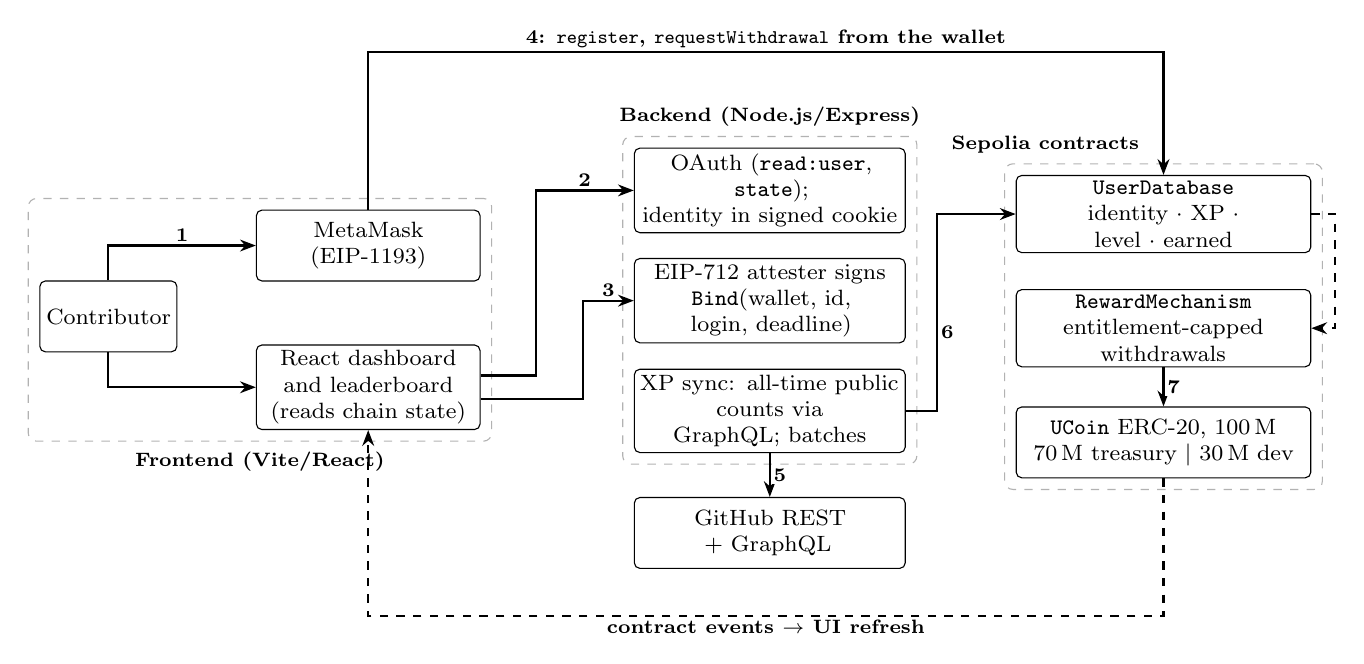
\begin{tikzpicture}[
  font=\footnotesize,
  box/.style={draw, rounded corners=2pt, align=center, minimum height=9mm, text width=#1, inner sep=2pt, fill=white},
  box/.default=27mm,
  lay/.style={draw=gray!60, dashed, rounded corners=3pt, inner sep=4pt},
  arr/.style={-{Stealth[length=2mm]}, thick},
  num/.style={font=\scriptsize\bfseries, fill=white, inner sep=1pt}]
\node[box=16mm] (user) at (0,0) {Contributor};
\node[box] (mm) at (3.3,0.9) {MetaMask\\(EIP-1193)};
\node[box] (ui) at (3.3,-0.9) {React dashboard\\and leaderboard\\(reads chain state)};
\node[box=33mm] (oauth) at (8.4,1.6) {OAuth (\texttt{read:user}, \texttt{state});\\identity in signed cookie};
\node[box=33mm] (att) at (8.4,0.2) {EIP-712 attester signs\\\texttt{Bind}(wallet, id, login, deadline)};
\node[box=33mm] (sync) at (8.4,-1.2) {XP sync: all-time public\\counts via GraphQL; batches};
\node[box=33mm] (gh) at (8.4,-2.75) {GitHub REST + GraphQL};
\node[box=36mm] (db) at (13.4,1.3) {\texttt{UserDatabase}\\identity $\cdot$ XP $\cdot$ level $\cdot$ earned};
\node[box=36mm] (rm) at (13.4,-0.15) {\texttt{RewardMechanism}\\entitlement-capped withdrawals};
\node[box=36mm] (tok) at (13.4,-1.6) {\texttt{UCoin} ERC-20, 100\,M\\70\,M treasury $\mid$ 30\,M dev};
\begin{scope}[on background layer]
\node[lay, fit=(user)(mm)(ui), label={[font=\scriptsize\bfseries]below:Frontend (Vite/React)}] {};
\node[lay, fit=(oauth)(att)(sync), label={[font=\scriptsize\bfseries]above:Backend (Node.js/Express)}] {};
\node[lay, fit=(db)(rm)(tok), label={[font=\scriptsize\bfseries, xshift=-15mm]above:Sepolia contracts}] {};
\end{scope}
\draw[arr] (user) |- node[num, pos=0.75, above]{1} (mm.west);
\draw[arr] (user) |- (ui.west);
\draw[arr] ([yshift=1.5mm]ui.east) -- ++(0.7,0) |- node[num, pos=0.75, above]{2} (oauth.west);
\draw[arr] ([yshift=-1.5mm]ui.east) -- ++(1.3,0) |- node[num, pos=0.75, above]{3} (att.west);
\draw[arr] (mm.north) -- ++(0,2.0) -| node[num, pos=0.25, above]{4: \texttt{register}, \texttt{requestWithdrawal} from the wallet} (db.north);
\draw[arr] (sync) -- node[num, right]{5} (gh);
\draw[arr] (sync.east) -- ++(0.4,0) |- node[num, pos=0.2, right]{6} (db.west);
\draw[arr] (rm) -- node[num, right]{7} (tok);
\draw[arr, dashed] (db.east) -- ++(0.3,0) |- (rm.east);
\draw[arr, dashed] (tok.south) -- ++(0,-1.75) -| node[num, pos=0.25, below]{contract events $\rightarrow$ UI refresh} (ui.south);
\end{tikzpicture}}
\caption{BlockSource architecture. (1) The wallet connects. (2) GitHub OAuth establishes the numeric account id; the token is discarded. (3) The backend signs a binding attestation. (4) The user calls \texttt{register} from the wallet; withdrawals are also sent from the wallet. (5) The sync job counts all-time public contributions and (6) submits \texttt{syncXP}/\texttt{syncXPBatch}. (7) \texttt{RewardMechanism} reads \emph{earned} from \texttt{UserDatabase} (dashed) and pays from the UCoin treasury it deployed. Contract events refresh the UI.}
\label{fig:arch}
\end{figure*}

\textit{Identity binding.} After OAuth, the backend knows the user's immutable numeric GitHub id and current login. On request it signs $\mathrm{Bind}(\mathit{wallet}, \mathit{githubId}, \mathit{login}, \mathit{deadline})$ with the attester key under the contract's EIP-712 domain, which fixes the application name, chain id and contract address. The user submits \texttt{register} from the named wallet. The contract recovers the signer, checks \texttt{ATTESTER\_ROLE}, and rejects a second wallet for the id or a second id for the wallet. Because \texttt{msg.sender} is inside the signed message, an attestation seen in the mempool cannot be replayed from another wallet; the deadline (10 minutes by default) limits the damage of a leaked signature; and revoking the attester role voids all outstanding attestations. This closes F3 for accounts, though one person can still own several GitHub accounts~\cite{douceur2002sybil,siddarth2020watchmen}.

\textit{Counting contributions.} The sync job resolves the current login from the id (\texttt{GET /user/\{id\}}, so renames are harmless), then sends one GraphQL request with one aliased \texttt{contributionsCollection} per calendar year since the account was created, because a collection spans at most a year~\cite{githubdocs}. It sums four counters per year: commits, issues, pull requests and pull-request reviews. Only public contributions are counted, with a server token that has no scopes, so the number does not depend on whose token is used (X1) and anyone can reproduce it. The login is passed as a GraphQL variable (X3).

\textit{Monotonic sync.} \texttt{syncXP(user, count)} sets $\XP = 50 \cdot \mathit{count}$ only if that exceeds the stored value. This one rule makes the sync idempotent (sending the same count twice is a no-op), order-insensitive (an old count arriving late is ignored), and safe against a count that shrinks when a user deletes a repository (F4). When XP rises, the contract computes the new level by Proposition~\ref{prop:inverse}, adds the rewards for every crossed level to \emph{earned}, and emits \texttt{LevelUp}. A batch form takes up to a few hundred users per transaction. The backend syncs a user on demand (rate-limited to once per 10 minutes) and all users every six hours.

\textit{Withdrawals.} \texttt{RewardMechanism} reads \emph{earned} and the active flag from \texttt{UserDatabase} and keeps \texttt{claimed[user]} itself. A request must satisfy $0 < a \le \mathit{earned} - \mathit{claimed}$; if $a \le$ \texttt{instantLimit} it is paid at once, otherwise it waits as a single pending request that the owner approves or rejects and the user can cancel. Hence for every user $\mathit{claimed} + \mathit{pending} \le \mathit{earned}$ at all times, and summed over users $\sum \mathit{earned} \le$ \texttt{rewardBudget} $=$ treasury, so the treasury cannot be overdrawn (F2, F6). State is written before the token transfer, and the token is OpenZeppelin's ERC-20 without transfer hooks, so the prototype's \texttt{ReentrancyGuard} is unnecessary~\cite{atzei2017survey,luu2016smarter}.

\textit{Storage layout.} A user occupies one 256-bit slot: \texttt{uint64 githubId}, \texttt{uint32 xp}, \texttt{uint8 level}, \texttt{uint96 earned}, \texttt{uint40 lastSync}, \texttt{bool suspended} (248 bits); a pending withdrawal (\texttt{uint96}, \texttt{bool}) fits in one more. The login is stored once in a separate mapping for display. Suspension replaces deletion (F7), and \texttt{getUsers(offset, limit)} replaces the unbounded \texttt{getAllUsers} (F8).

\textit{Frontend.} The dashboard now shows what the contracts say: XP, level and \emph{earned} from \texttt{UserDatabase}, \emph{claimed} and \emph{available} from \texttt{RewardMechanism}. It asks the wallet to switch to the configured chain before any transaction, decodes custom-error reverts into messages, and refreshes on contract events instead of the prototype's 15-second and 30-second polling. Contract addresses come from build-time environment variables instead of source code. The leaderboard pages through \texttt{getUsers} and ranks by on-chain XP, so every visitor sees the same order (X2).

%======================================================================
\section{Evaluation}\label{sec:eval}
%======================================================================

\subsection{Testbed and methodology}
Contracts run on the Hardhat EDR network (Cancun rules). The prototype's sources are compiled as deployed (solc~0.8.20, optimizer off); BlockSource uses solc~0.8.26 with the optimizer at 200 runs. Gas is a deterministic function of bytecode, fork rules and state, so local figures should match on-chain receipts for the same calls; Section~\ref{sec:validate} checks this. US-dollar figures assume ETH at US\$2{,}725 (early October 2026) and scale linearly in price and gas price; we price at 0.5\,gwei, close to 2026's mainnet daily averages~\cite{ethorg2026}, and at 15 and 40\,gwei. Backend timings were taken on a 2-vCPU Intel Xeon at 2.1\,GHz with Node.js~22. We could not call GitHub's GraphQL API from the test environment, so GitHub responses in backend tests are recorded fixtures.

\subsection{Functional verification}
The contract suite has 71 Hardhat tests: 8 reproduce the prototype's findings, 62 cover BlockSource (tokenomics, progression maths, binding, sync, suspension, pagination, withdrawals, solvency and access control), and one runs the backend's attestation and sync code against the BlockSource contracts end to end. All pass, with 100\% statement, branch, function and line coverage of the three BlockSource contracts under \texttt{solidity-coverage}. The backend has 9 further tests covering year-by-year counting, GraphQL variable handling, id mismatch, OAuth \texttt{state} rejection, the absence of tokens in redirects, attestation recovery, the sync cooldown, and batch selection that skips suspended and unchanged users. The frontend builds with Vite and passes ESLint (React hooks rules) without errors.

\subsection{Validating gas measurement against Sepolia}\label{sec:validate}
Sepolia receipts give gas used as fee divided by gas price. Table~\ref{tab:validate} compares them with the same calls on a local build of the prototype. Registration and withdrawal requests match within the rounding of the explorer's fee display. Approvals are 0.5--0.6\% higher locally; the deployed \texttt{RewardMechanism} is unverified, so the repository source may not be byte-identical to it, and function dispatch order alone can shift gas by a few hundred units. We take the local environment as accurate to within 1\% for the comparisons that follow.

\begin{table}[t]
\centering
\caption{Prototype gas: local re-execution vs.\ Sepolia receipts}
\label{tab:validate}
\footnotesize
\setlength{\tabcolsep}{3pt}
\begin{tabular}{@{}lrrr@{}}
\toprule
\textbf{Call} & \textbf{Local} & \textbf{Sepolia (range)} & \textbf{Diff.}\\
\midrule
\texttt{setUser}, first user & 121{,}760 & 121{,}767 & 0.0\%\\
\texttt{setUser}, later users & 124{,}548 & 124{,}511--124{,}571 & 0.0\%\\
\texttt{requestWithdrawal} & 68{,}019 & 68{,}013--68{,}019 & 0.0\%\\
\texttt{approveWithdrawal}, new holder & 64{,}992 & 64{,}657--64{,}660 & +0.5\%\\
\texttt{approveWithdrawal}, existing & 48{,}234 & 47{,}966--47{,}968 & +0.6\%\\
\bottomrule
\end{tabular}
\end{table}

\subsection{Gas: prototype versus BlockSource}\label{sec:gas}
Table~\ref{tab:gas} compares the two designs. Registration costs 3.5\% more in BlockSource because it verifies an ECDSA signature and stores a reverse mapping, which buys the identity binding. A single-user XP sync costs 33.7\% less than the prototype's \texttt{updateUserXP} although it also computes the level, because the profile is one packed slot; with a level-up it costs 42{,}096 gas. In batches of 100 the cost falls to 14{,}004 gas per user (Fig.~\ref{fig:batch}). A withdrawal request is 18.0\% cheaper. The first payout to a user costs 34.6\% more because it creates \texttt{claimed[user]}, a zero-to-nonzero store of about 22{,}100 gas; this is the price of moving the prototype's \texttt{localStorage} entry on chain, and it is paid once per user. Deploying BlockSource takes 3.81\,M gas against 4.79\,M for the prototype (excluding the prototype's separate treasury funding transfer), because \texttt{RewardMechanism} creates and funds UCoin in its constructor.

\begin{table}[t]
\centering
\caption{Gas per operation; US\$ cost of BlockSource calls (ETH = US\$2{,}725)}
\label{tab:gas}
\scriptsize
\setlength{\tabcolsep}{2.4pt}
\begin{tabular}{@{}lrrrrrr@{}}
\toprule
& \textbf{Proto-} & \textbf{Block-} & & \multicolumn{3}{c}{\textbf{US\$ at gwei}}\\
\cmidrule(l){5-7}
\textbf{Operation} & \textbf{type} & \textbf{Source} & \textbf{$\Delta$} & \textbf{0.5} & \textbf{15} & \textbf{40}\\
\midrule
Register & 124{,}548 & 128{,}959 & +3.5\% & 0.18 & 5.27 & 14.06\\
XP update, single user & 50{,}731 & 33{,}611 & $-$33.7\% & 0.05 & 1.37 & 3.66\\
\quad with level-up & -- & 42{,}096 & & 0.06 & 1.72 & 4.59\\
\quad batch of 100, per user & -- & 14{,}004 & & 0.02 & 0.57 & 1.53\\
\quad same count again (no-op) & -- & 27{,}131 & & 0.04 & 1.11 & 2.96\\
\texttt{requestWithdrawal} & 68{,}019 & 55{,}767 & $-$18.0\% & 0.08 & 2.28 & 6.08\\
Approve, first payout to user & 64{,}992 & 87{,}468 & +34.6\% & 0.12 & 3.58 & 9.53\\
Approve, later payout & 48{,}234 & 53{,}268 & +10.4\% & 0.07 & 2.18 & 5.81\\
Request paid instantly & -- & 56{,}383 & & 0.08 & 2.30 & 6.15\\
Reject & 29{,}222 & 26{,}449 & $-$9.5\% & 0.04 & 1.08 & 2.88\\
\bottomrule
\end{tabular}
\end{table}

\begin{figure}[t]
\centering
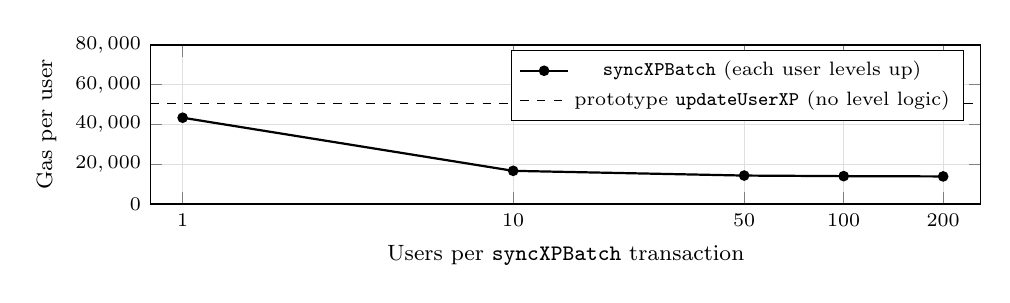
\begin{tikzpicture}
\begin{axis}[width=\columnwidth, height=3.6cm, xmode=log, log basis x=10,
  xlabel={Users per \texttt{syncXPBatch} transaction}, ylabel={Gas per user},
  ymin=0, ymax=80000, xmin=0.8, xmax=260,
  xtick={1,10,50,100,200}, xticklabels={1,10,50,100,200},
  yticklabel style={/pgf/number format/fixed,/pgf/number format/1000 sep={,}},
  scaled y ticks=false, grid=major, grid style={gray!25},
  legend style={font=\scriptsize, at={(0.98,0.97)}, anchor=north east},
  tick label style={font=\scriptsize}, label style={font=\footnotesize}]
\addplot[thick, mark=*, mark size=1.5pt] coordinates {(1,43414)(10,16674)(50,14298)(100,14004)(200,13864)};
\addlegendentry{\texttt{syncXPBatch} (each user levels up)}
\addplot[dashed, domain=0.8:260] {50731};
\addlegendentry{prototype \texttt{updateUserXP} (no level logic)}
\end{axis}
\end{tikzpicture}
\caption{Per-user gas of a batched XP sync. Every user in the batch crosses one level.}
\label{fig:batch}
\end{figure}

The cost model differs from per-event designs in a useful way. A sync carries a \emph{count}, so its gas does not depend on how many contributions the count covers. A user who made 30 contributions since the last sync costs the same 14{,}004 gas in a batch as one who made one. Deduplication is free because the monotonic rule replaces a per-contribution ``seen'' map, which in a per-event design costs a 22{,}100-gas store for every contribution.

\subsection{Burst throughput}
We registered 500 users, gave each some history, then let all 500 gain five contributions at once (no level is crossed) and drained the mempool with automatic mining off (Table~\ref{tab:burst}). Submitting one \texttt{syncXP} per user used 16.8\,M gas; five \texttt{syncXPBatch} calls of 100 users used 5.2\,M, 69\% less, or 2{,}088 gas per contribution. Both fit in one block at 30, 36 and 60\,M gas limits, and every user ended at the same XP and level in both modes. If the system may use 5\% of a 60\,M-gas block (3\,M gas per 12\,s slot), batched syncs cover about 287 users per slot, so a six-hourly sweep of 100{,}000 active users needs roughly 350 slots, or 70 minutes.

\begin{table}[t]
\centering
\caption{500 users with new contributions at once}
\label{tab:burst}
\footnotesize
\setlength{\tabcolsep}{3.5pt}
\begin{tabular}{@{}lrrrr@{}}
\toprule
\textbf{Mode} & \textbf{Txs} & \textbf{Total gas} & \textbf{Gas/user} & \textbf{Blocks}\\
\midrule
One \texttt{syncXP} per user & 500 & 16{,}816{,}984 & 33{,}634 & 1\\
\texttt{syncXPBatch} of 100 & 5 & 5{,}218{,}883 & 10{,}438 & 1\\
\bottomrule
\end{tabular}
\end{table}

\subsection{Latency}
Off-chain work is small. On the test machine, signing a binding attestation takes 6.0\,ms on average (p95 8.1\,ms), parsing a four-year GraphQL response 0.01\,ms, and encoding and signing a 100-user batch transaction 8.7\,ms (p95 11.4\,ms). The GitHub API round trip, which we could not measure here, and slot timing dominate. Ethereum produces a block every 12\,s~\cite{buterin2020gasper}; a uniformly timed submission waits on average half a slot plus the propagation margin, about 7--11\,s to inclusion in a Monte-Carlo slot model with 1--3\,s submission delay and up to 5\% empty slots, and economic finality takes about 12.8 minutes. A user who presses ``Sync now'' therefore sees new XP in roughly one GitHub round trip plus one slot. Users who do nothing are updated by the six-hourly sweep, so the worst-case staleness of passive users is six hours plus the sweep time; the prototype, by contrast, never updated on-chain XP at all.

\subsection{Treasury capacity}
Table~\ref{tab:prog} and Fig.~\ref{fig:prog} apply Proposition~\ref{prop:emission}. The prototype's supply would have paid level~20 to about 2{,}800 contributors and level~100 to fewer than five; the treasury would have run dry at the scale of a single mid-sized open-source community. With $10^{8}$~UCN, BlockSource carries 283{,}269 contributors to the Reviewer level.

\begin{table}[t]
\centering
\caption{Progression and users fundable from the treasury (prototype: 0.7\,M UCN; BlockSource: 70\,M UCN)}
\label{tab:prog}
\footnotesize
\setlength{\tabcolsep}{2.6pt}
\begin{tabular}{@{}rrrrrr@{}}
\toprule
& & & & \multicolumn{2}{c}{\textbf{Users fundable to $L$}}\\
\cmidrule(l){5-6}
\textbf{$L$} & \textbf{XP} & \textbf{Contrib.} & \textbf{$S(L)$ UCN} & \textbf{Prototype} & \textbf{BlockSource}\\
\midrule
1 & 100 & 2 & 5.4 & 129{,}630 & 12{,}962{,}963\\
5 & 1{,}500 & 30 & 31.7 & 22{,}096 & 2{,}209{,}621\\
10 & 5{,}500 & 110 & 78.2 & 8{,}948 & 894{,}827\\
20 & 21{,}000 & 420 & 247.1 & 2{,}833 & 283{,}269\\
50 & 127{,}500 & 2{,}550 & 3{,}098.4 & 226 & 22{,}593\\
100 & 505{,}000 & 10{,}100 & 148{,}416.4 & 4.7 & 471.6\\
\bottomrule
\end{tabular}
\end{table}

\begin{figure}[t]
\centering
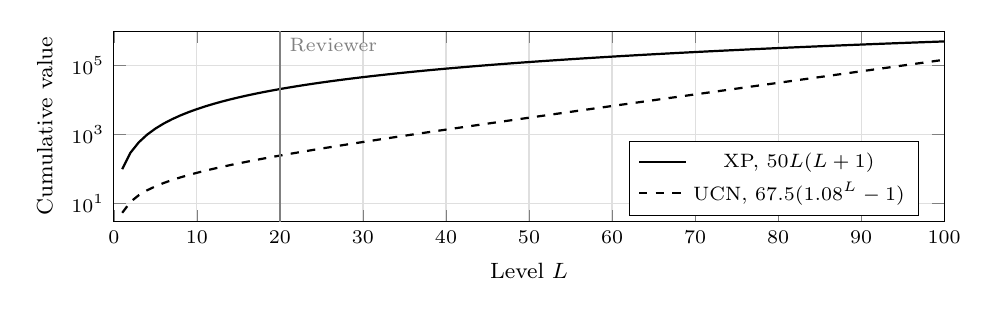
\begin{tikzpicture}
\begin{semilogyaxis}[width=\columnwidth, height=4.0cm,
  xlabel={Level $L$}, ylabel={Cumulative value},
  xmin=0, xmax=100, ymin=3, ymax=1e6, grid=major, grid style={gray!25},
  legend style={font=\scriptsize, at={(0.97,0.03)}, anchor=south east},
  tick label style={font=\scriptsize}, label style={font=\footnotesize}]
\addplot[thick, domain=1:100, samples=100] {50*x*(x+1)};
\addlegendentry{XP, $50L(L+1)$}
\addplot[thick, dashed, domain=1:100, samples=100] {67.5*(1.08^x-1)};
\addlegendentry{UCN, $67.5(1.08^{L}-1)$}
\draw[gray] (axis cs:20,3) -- (axis cs:20,1e6) node[pos=0.93, right, font=\scriptsize]{Reviewer};
\end{semilogyaxis}
\end{tikzpicture}
\caption{Cumulative XP and cumulative UCN by level; the vertical line marks Reviewer promotion at level~20.}
\label{fig:prog}
\end{figure}

%======================================================================
\section{Discussion and Limitations}\label{sec:discussion}
%======================================================================

\subsection{What the prototype taught us}
Three lessons from the prototype generalise to other incentive DApps. First, a limit enforced only in the user interface is not a limit: F2 and F6 both come from treating the dashboard's arithmetic as the system's rules. Second, a role that no code path exercises (\texttt{XP\_UPDATER\_ROLE}) is a sign that a component is missing, and the Sepolia history confirms it. Third, wherever a number is shown to users, it should be the number the contract will act on; the prototype's leaderboard, dashboard and contracts each had their own idea of a user's standing.

\subsection{Storage and decentralisation}
Keeping XP and entitlements on chain buys auditability and lets anyone rebuild the leaderboard from events. It also makes each sync cost gas, which at 15--40\,gwei on L1 is \$0.57--1.53 per user even in batches. Two moves would cut this by one to two orders of magnitude without changing the contracts: deploying them on an optimistic or validity rollup~\cite{kalodner2018arbitrum,thibault2022rollups}, where most Ethereum activity already runs~\cite{ethorg2026}, and posting a Merkle root of all counts per sweep, with per-user proofs submitted only when a user withdraws. Rich metadata such as streaks and review text belongs in an indexer or on IPFS~\cite{benet2014ipfs}.

\subsection{Quality versus quantity}\label{sec:gaming}
A fixed 50~XP per contribution makes XP a count, and counts invite Goodhart's law~\cite{strathern1997goodhart}. Commit splitting, trivial issues, self-reviews in throwaway repositories and duplicate GitHub accounts all raise the count. Proposition~\ref{prop:yield} sharpens the concern: the yield past level~13 rises to 55~UCN per contribution at level~100, a level that takes an honest contributor decades and a script days. GitHub data is also a noisy measure of work~\cite{kalliamvakou2014perils}, and visible counters change when people work~\cite{moldon2021gamification}. BlockSource does not solve this. It makes counts public and reproducible, so abuse is visible, and it gives administrators suspension and payout review. Future work should weight contributions by review outcome rather than count them~\cite{bacchelli2013review,gousios2014pull}, cap XP per period, index the reward schedule to the remaining treasury, and move these parameters to DAO governance~\cite{hassan2021dao,wang2019dao}. A token's value also depends on adoption, which a schedule alone does not create~\cite{cong2021tokenomics}.

\subsection{Threats to validity}
Our prototype evidence is a seven-user testnet deployment; it shows what the system did, not how a large community would behave. The 0.5--0.6\% gap in approval gas may come from a deployed bytecode that differs from the repository. GitHub responses in backend tests are fixtures, and we did not measure GitHub API latency. Contribution counts follow GitHub's own counting rules, which, for example, credit commits only on default branches. We ran no user study and make no claim that XP, levels or titles change contribution behaviour~\cite{hamari2014gamification,anderson2013badges}.

%======================================================================
\section{Conclusion and Future Work}\label{sec:conclusion}
%======================================================================
The BlockSource prototype demonstrated the idea of turning GitHub activity into on-chain levels and tokens, and its Sepolia record shows a team using it. It also showed where prototypes of this kind fail: the browser held the rules, the contracts held the money, and nothing connected them. The hardened design moves identity, XP, levels, entitlements and claims on chain, binds one GitHub account to one wallet, and replaces client-side XP with a monotonic, publicly reproducible count. The contract suite passes 71 tests with full coverage, local gas agrees with Sepolia within 0.6\%, batched syncs cost 14{,}004 gas per user, and a $10^{8}$-UCN supply funds a hundred times more contributors than the prototype's.

Next steps follow from the limitations: deploy the hardened contracts on Sepolia and then on an L2; replace the single attester with several independent oracle nodes or authenticated TLS data~\cite{zhang2016towncrier}, so that no one key decides a count; weight XP by review outcome; add GitLab and Bitbucket through a forge prefix on the account id; and put reward parameters and payout review under DAO control.

\bibliographystyle{IEEEtran}
\bibliography{refs}

\end{document}
